%%%%%%%%%%%%%%%%%%%%%%%%%%%%%%%%%%%%%%%%%%%%%%%%%%%%%%%%%%%%%%%%%%%%%%%
%% COMPANION NOTE D: Selection Rules for Neutron Beta Decay in EDC
%% A 5D Topological Necessity of a Neutral Mode with Fifth Momentum
%%
%% Companion D to Paper 3 (NJSR Edition)
%% Build: XeLaTeX (Unicode)
%%
%% Author: Igor Grčman
%% Date: January 2026
%% Status: Reviewer-grade, epistemic cleanup
%%%%%%%%%%%%%%%%%%%%%%%%%%%%%%%%%%%%%%%%%%%%%%%%%%%%%%%%%%%%%%%%%%%%%%%

\documentclass[11pt,a4paper]{article}

%% ===== PACKAGES =====
\usepackage{fontspec}
\usepackage{amsmath,amssymb,amsthm}
\usepackage{tikz}
\usepackage{tcolorbox}
\tcbuselibrary{breakable,theorems}
\usepackage{array}
\usepackage{booktabs}
\usepackage{geometry}
\usepackage[colorlinks=true,linkcolor=blue,citecolor=blue,urlcolor=blue]{hyperref}
\usepackage{xcolor}
\usepackage{enumitem}
\usepackage[style=numeric-comp,sorting=none,backend=biber]{biblatex}
\addbibresource{refs_topology_note.bib}

\geometry{margin=1in}

%% ===== FONTS (fallback to default if TeX Gyre not available) =====
\IfFontExistsTF{TeX Gyre Termes}{%
  \setmainfont{TeX Gyre Termes}
  \setsansfont{TeX Gyre Heros}
}{%
  % Fallback to system fonts
  \setmainfont{Times New Roman}[Ligatures=TeX]
  \setsansfont{Helvetica}
}

%% ===== CUSTOM COLORS =====
\definecolor{braneblue}{RGB}{0,100,180}
\definecolor{plenumgray}{RGB}{100,100,100}
\definecolor{electronblue}{RGB}{0,80,160}
\definecolor{neutrinoorange}{RGB}{220,120,0}
\definecolor{taggreen}{RGB}{0,120,60}
\definecolor{tagred}{RGB}{180,0,0}
\definecolor{tagyellow}{RGB}{180,140,0}

%% ===== THEOREM ENVIRONMENTS =====
\newtheorem{proposition}{Proposition}
\newtheorem{theorem}{Theorem}
\newtheorem{lemma}{Lemma}
\theoremstyle{definition}
\newtheorem{definition}{Definition}
\theoremstyle{remark}
\newtheorem*{remark}{Remark}

%% ===== EPISTEMIC TAG COMMANDS =====
\newcommand{\tagI}{\textcolor{taggreen}{\textbf{[I]}}}
\newcommand{\tagDef}{\textcolor{blue}{\textbf{[Def]}}}
\newcommand{\tagP}{\textcolor{tagyellow}{\textbf{[P]}}}
\newcommand{\tagDc}{\textcolor{taggreen}{\textbf{[Dc]}}}
\newcommand{\tagDer}{\textcolor{taggreen}{\textbf{[Der]}}}
\newcommand{\tagOPEN}{\textcolor{tagred}{\textbf{[OPEN]}}}
\newcommand{\tagBL}{\textcolor{gray}{\textbf{[BL]}}}

%% ===== TITLE =====
\title{\textbf{Selection Rules for Neutron $\beta^-$ Decay\\in Elastic Diffusive Cosmology}\\[0.5em]
\large A 5D Topological Necessity of a Neutral Mode with $p^\xi \neq 0$\\[0.3em]
\normalsize (Companion D to Paper~3: NJSR Edition)}
\author{Igor Gr\v{c}man}
\date{January 2026\\[0.5em]
\small Repository: \href{https://github.com/igorgrcman/elastic-diffusive-cosmology}{github.com/igorgrcman/elastic-diffusive-cosmology}\\[0.2em]
\footnotesize (Public artifacts for this paper are in the \texttt{edc\_papers} folder.)}

\begin{document}

\maketitle

\begin{center}
\small\textbf{Related Documents:}\\[0.1cm]
\footnotesize
\textbf{Companions:}\\
\end{center}

%%%%%%%%%%%%%%%%%%%%%%%%%%%%%%%%%%%%%%%%%%%%%%%%%%%%%%%%%%%%%%%%%%%%%%%
%% ABSTRACT
%%%%%%%%%%%%%%%%%%%%%%%%%%%%%%%%%%%%%%%%%%%%%%%%%%%%%%%%%%%%%%%%%%%%%%%

\begin{abstract}
\noindent
This companion note establishes the \emph{selection rules} for neutron $\beta^-$ decay within the 5D Elastic Diffusive Cosmology (EDC) framework. We derive, from topological charge conservation and kinematic constraints, that the decay must produce exactly two outputs: (i)~a brane-bound excitation carrying $Q=-1$ (topologically confined to $\xi = 0$), and (ii)~a neutral mode with nonzero fifth momentum $p^\xi \neq 0$. \textbf{Both outputs are created on the brane}; the distinction is kinematic---the neutral mode can carry momentum in the fifth dimension while the charged mode cannot. The note addresses channel legality and budget bookkeeping only; it does \emph{not} compute the decay lifetime $\tau_n$ (treated in Paper~3 via WKB methods). No Standard Model dynamical parameters are used as inputs; particle labels appear only as observational identifiers. All conclusions are conditional on the stated assumptions.
\end{abstract}

%%%%%%%%%%%%%%%%%%%%%%%%%%%%%%%%%%%%%%%%%%%%%%%%%%%%%%%%%%%%%%%%%%%%%%%
\section{Introduction}
%%%%%%%%%%%%%%%%%%%%%%%%%%%%%%%%%%%%%%%%%%%%%%%%%%%%%%%%%%%%%%%%%%%%%%%

Neutron $\beta^-$ decay is one of the most precisely measured processes in nuclear physics. In the Standard Model, it is mediated by $W$-boson exchange within the electroweak framework. This note takes a different approach: we ask what constraints on the decay channel arise from the 5D topological structure of Elastic Diffusive Cosmology (EDC), \emph{independent} of any Standard Model mechanism.

\subsection{Scope and Two-Sided Presentation}

Throughout this note, we adopt a \textbf{two-sided rule}:
\begin{center}
\begin{tabular}{|c|c|}
\hline
\textbf{Left side: 5D EDC cause} & \textbf{Right side: 3D observational evidence} \\
\hline
Topological constraint & Measured quantity \tagBL{} \\
Conservation law \tagDc{}/\tagDer{} & Experimental signature \\
\hline
\end{tabular}
\end{center}

This separation ensures that Standard Model facts appear only as \emph{observational targets} to be matched, never as theoretical inputs to the derivation.

\subsection{What This Note Does and Does Not Do}

\begin{tcolorbox}[colback=yellow!5!white, colframe=yellow!50!black, title=\textbf{Scope Declaration}]
\textbf{This note addresses:}
\begin{itemize}[nosep]
  \item Channel selection rules (which output configurations are permitted)
  \item Charge, winding, and momentum budget bookkeeping
  \item The necessity of a neutral mode with $p^\xi \neq 0$ (``antineutrino'')
\end{itemize}

\textbf{This note does NOT:}
\begin{itemize}[nosep]
  \item Compute the neutron lifetime $\tau_n$ (see the main paper \cite{paper3})
  \item Derive SM coupling constants ($G_F$, $V_{ud}$, etc.)
  \item Model collider cross-sections or high-energy processes
  \item Derive the effective Lagrangian $\mathcal{L}_{\text{eff}}$ from first principles (see companion note \cite{Leff_companion})
\end{itemize}
\end{tcolorbox}

%%%%%%%%%%%%%%%%%%%%%%%%%%%%%%%%%%%%%%%%%%%%%%%%%%%%%%%%%%%%%%%%%%%%%%%
\section{Assumptions, Definitions, and Epistemic Legend}
%%%%%%%%%%%%%%%%%%%%%%%%%%%%%%%%%%%%%%%%%%%%%%%%%%%%%%%%%%%%%%%%%%%%%%%

\subsection{Epistemic Tag Legend}

All statements in this note carry explicit epistemic tags:

\begin{center}
\renewcommand{\arraystretch}{1.3}
\begin{tabular}{|c|l|l|}
\hline
\textbf{Tag} & \textbf{Meaning} & \textbf{Example} \\
\hline
\tagI{} & Empirical input (observation) & Continuous $e^-$ spectrum \\
\tagDef{} & Definition introduced here & Collective coordinate $q$ \\
\tagP{} & Working hypothesis & Junction unwinding chirality \\
\tagDc{} & Decisively constrained (conditional) & Mode classification \\
\tagDer{} & Derived within stated equations & Charge budget \\
\tagOPEN{} & Deferred / not yet derived & Junction chirality origin \\
\tagBL{} & Baseline observational fact & $Q_{\text{decay}} = 1.293$ MeV \\
\hline
\end{tabular}
\end{center}

\subsection{Assumption Box}

\begin{tcolorbox}[colback=blue!5!white, colframe=blue!50!black, title=\textbf{Assumptions for This Note}]

\textbf{Geometric/Topological Assumptions:}
\begin{enumerate}[label=\textbf{A\arabic*}., nosep]
  \item \tagP{} The observable universe is a 3-brane $\Sigma$ embedded in 5D spacetime $\mathcal{M}_5$.
  \item \tagP{} Baryons are Y-junctions of three flux tubes meeting on $\Sigma$.
  \item \tagDef{} Electric charge $Q$ is a topological winding number: $Q = \frac{1}{2\pi}\oint A_\phi\,d\phi$.
  \item \tagP{} Topological winding is conserved across decay processes.
  \item \tagP{} Fifth momentum $p^\xi$ is conserved (with Plenum recoil absorption).
\end{enumerate}

\textbf{Empirical Inputs:}
\begin{enumerate}[label=\textbf{I\arabic*}., nosep]
  \item \tagI{} The electron spectrum in $\beta^-$ decay is continuous (not monoenergetic).
  \item \tagI{} Neutrinos/antineutrinos are electrically neutral ($Q_\nu = 0$).
  \item \tagI{} The decay releases $Q_{\text{decay}} = 1.293$ MeV \tagBL{}.
  \item \tagI{} The proton carries charge $Q_p = +1$; neutron carries $Q_n = 0$ \tagBL{}.
\end{enumerate}

\textbf{Classification Convention:}
\begin{enumerate}[label=\textbf{C\arabic*}., nosep]
  \item \tagDef{}/\tagP{} Particle vs.\ antiparticle is distinguished by the combination $(h_5, \text{sign}(p^\xi))$ where $h_5$ is the 5D helicity.
\end{enumerate}

\end{tcolorbox}

%%%%%%%%%%%%%%%%%%%%%%%%%%%%%%%%%%%%%%%%%%%%%%%%%%%%%%%%%%%%%%%%%%%%%%%
\section{The 5D Stage and Topological Defects}
%%%%%%%%%%%%%%%%%%%%%%%%%%%%%%%%%%%%%%%%%%%%%%%%%%%%%%%%%%%%%%%%%%%%%%%

\subsection{Spacetime Structure}

In EDC, spacetime is 5-dimensional:
\begin{equation}
\mathcal{M}_5 = \{(x^\mu, \xi) : x^\mu \in \mathbb{R}^{1,3},\; \xi \in \mathbb{R}\} \tag{\tagP{}}
\end{equation}

The brane $\Sigma$ at $\xi = 0$ hosts observable matter. The bulk ($\xi > 0$) is the Plenum, an energy reservoir with positive pressure $P_{\text{bulk}} > 0$.

\begin{center}
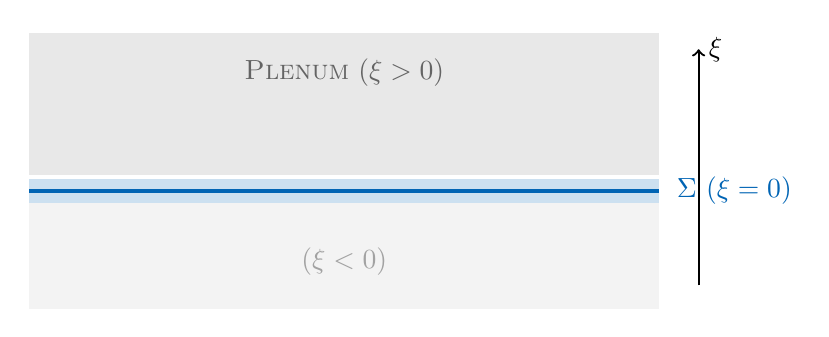
\begin{tikzpicture}[scale=1.0]
  \fill[plenumgray!15] (-4,0.2) rectangle (4,2);
  \node[plenumgray] at (0,1.5) {\textsc{Plenum} ($\xi > 0$)};
  \fill[braneblue!20] (-4,-0.15) rectangle (4,0.15);
  \draw[very thick, braneblue] (-4,0) -- (4,0);
  \node[braneblue, right] at (4.1,0) {$\Sigma$ ($\xi=0$)};
  \fill[plenumgray!8] (-4,-1.5) rectangle (4,-0.15);
  \node[plenumgray!60] at (0,-0.9) {($\xi < 0$)};
  \draw[->, thick] (4.5,-1.2) -- (4.5,1.8) node[right] {$\xi$};
\end{tikzpicture}
\end{center}

\subsection{Baryons as Y-Junctions}

\begin{definition}[Y-Junction] \tagDef{}
A baryon is a Y-junction where three flux tubes meet on the brane $\Sigma$. The junction is characterized by three unit vectors $\hat{e}_1, \hat{e}_2, \hat{e}_3$ pointing along the flux tubes.
\end{definition}

\begin{definition}[Collective Coordinate $q$] \tagDef{}
The junction asymmetry is measured by:
\begin{equation}
q \equiv \frac{|\hat{e}_1 + \hat{e}_2 + \hat{e}_3|}{3} \in [0, 1]
\end{equation}
\begin{itemize}[nosep]
  \item $q = 0$: Symmetric Steiner configuration (120° angles) $\to$ proton (stable)
  \item $q = q_n \approx 0.31$: Asymmetric configuration $\to$ neutron (unstable)
\end{itemize}
\end{definition}

\begin{definition}[Topological Charge] \tagDef{}
Electric charge is defined as a topological winding number:
\begin{equation}
Q = \frac{1}{2\pi} \oint A_\phi \, d\phi \in \mathbb{Z}
\end{equation}
\end{definition}

\begin{center}
\begin{tabular}{|l|c|c|c|}
\hline
\textbf{Defect} & \textbf{$Q$} & \textbf{Baryonic $W$} & \textbf{Status} \\
\hline
Proton & $+1$ & $+1$ & Brane-bound \tagBL{} \\
Neutron & $0$ & $+1$ & Brane-bound \tagBL{} \\
Electron & $-1$ & $0$ & Brane-bound \tagBL{} \\
Neutral mode & $0$ & $0$ & $p^\xi \neq 0$ allowed \tagDc{} \\
\hline
\end{tabular}
\end{center}

\begin{tcolorbox}[colback=red!5!white, colframe=red!50!black, title=\textbf{Important Clarification: Where Particles Are Created}]
\textbf{All decay products are created on the brane ($\xi = 0$).}

The distinction between ``brane-bound'' and ``$p^\xi \neq 0$ allowed'' is \emph{kinematic}, not about origin:
\begin{itemize}[nosep]
  \item \textbf{Brane-bound} ($Q \neq 0$): Topological charge requires a localized core; the mode \emph{cannot} carry fifth momentum. It is confined to $\xi = 0$.
  \item \textbf{$p^\xi \neq 0$ allowed} ($Q = 0$): No topological obstruction; the mode \emph{can} carry momentum in the $\xi$-direction, even though it is created on the brane.
\end{itemize}

The antineutrino does not ``live in the bulk''---it is created on the brane like all other decay products. However, it can carry energy-momentum into the fifth dimension, which is why fifth-momentum conservation requires its existence.
\end{tcolorbox}

%%%%%%%%%%%%%%%%%%%%%%%%%%%%%%%%%%%%%%%%%%%%%%%%%%%%%%%%%%%%%%%%%%%%%%%
\section{Conserved Budgets Across the Membrane}
%%%%%%%%%%%%%%%%%%%%%%%%%%%%%%%%%%%%%%%%%%%%%%%%%%%%%%%%%%%%%%%%%%%%%%%

The decay process $n \to p + X$ must satisfy several conservation constraints. We analyze each budget systematically.

\subsection{Charge Budget}

\begin{proposition}[Charge Closure] \tagDer{}
The decay outputs must carry total charge $Q = -1$.
\end{proposition}

\begin{proof}
By charge conservation (Assumption A4):
\begin{equation}
Q_n = Q_p + \sum_i Q_i
\end{equation}
Substituting known values \tagBL{}:
\begin{equation}
0 = +1 + \sum_i Q_i \quad \Longrightarrow \quad \boxed{\sum_i Q_i = -1}
\end{equation}
\end{proof}

\textbf{Two-sided check:}
\begin{center}
\begin{tabular}{|c|c|}
\hline
\textbf{5D cause} & \textbf{3D evidence} \\
\hline
Winding conservation \tagDer{} & Electron carries $Q = -1$ \tagBL{} \\
\hline
\end{tabular}
\end{center}

\subsection{Baryonic Winding Budget}

\begin{proposition}[Winding Closure] \tagDer{}
The decay outputs carry no net baryonic winding.
\end{proposition}

\begin{proof}
\begin{equation}
W_n = W_p + \sum_i W_i \quad \Longrightarrow \quad +1 = +1 + \sum_i W_i \quad \Longrightarrow \quad \boxed{\sum_i W_i = 0}
\end{equation}
\end{proof}

\textbf{Implication:} Outputs are not baryons (leptons only).

\subsection{Kinematic/Spectral Constraint}

\begin{proposition}[Three-Body Necessity] \tagI{}/\tagDc{}
The decay cannot be a pure two-body process; a third channel is required.
\end{proposition}

\begin{proof}
Empirical input \textbf{I1}: The electron spectrum is continuous, not monoenergetic.

A two-body decay $n \to p + e^-$ would produce a monoenergetic electron with:
\begin{equation}
E_e = \frac{(m_n - m_p)^2 + m_e^2}{2m_n} c^2 \approx 1.29 \text{ MeV}
\end{equation}

The observed continuous spectrum \tagI{} rules out pure two-body kinematics. Therefore, a third participant is required to absorb the missing energy-momentum.
\end{proof}

\textbf{Two-sided check:}
\begin{center}
\begin{tabular}{|c|c|}
\hline
\textbf{5D cause} & \textbf{3D evidence} \\
\hline
Energy-momentum balance \tagDc{} & Continuous $e^-$ spectrum \tagI{} \\
\hline
\end{tabular}
\end{center}

\subsection{Fifth Momentum Budget}

\begin{proposition}[$p^\xi$ Balance] \tagDc{}/\tagP{}
Under Assumption A5, at least one output must have $p^\xi \neq 0$.
\end{proposition}

\begin{proof}
Fifth momentum conservation with Plenum recoil:
\begin{equation}
p^\xi_n = p^\xi_p + \sum_i p^\xi_i + \Delta p^\xi_{\text{Plenum}}
\end{equation}

Since neutron and proton are both brane-bound: $p^\xi_n = p^\xi_p = 0$.

If the Plenum absorbs nonzero recoil ($\Delta p^\xi_{\text{Plenum}} \neq 0$), then:
\begin{equation}
\sum_i p^\xi_i = -\Delta p^\xi_{\text{Plenum}} \neq 0 \quad \Longrightarrow \quad \boxed{\exists\, p^\xi_i \neq 0}
\end{equation}
\end{proof}

\textbf{Implication:} At least one output mode carries nonzero fifth momentum $p^\xi \neq 0$.

%%%%%%%%%%%%%%%%%%%%%%%%%%%%%%%%%%%%%%%%%%%%%%%%%%%%%%%%%%%%%%%%%%%%%%%
\section{Selection Rules: Formal Propositions}
%%%%%%%%%%%%%%%%%%%%%%%%%%%%%%%%%%%%%%%%%%%%%%%%%%%%%%%%%%%%%%%%%%%%%%%

\subsection{Mode Classification}

\begin{theorem}[Brane Localization] \tagDc{}
If $Q \neq 0$, then $p^\xi = 0$ (mode is brane-bound).
\end{theorem}

\begin{proof}
Within the stated assumptions:
\begin{enumerate}[nosep]
  \item Non-zero winding ($Q \neq 0$) requires a topological core.
  \item Cores are localized at brane junctions (by construction of defects).
  \item Bulk waves ($\xi > 0$) have no localized core structure.
  \item Therefore: $Q \neq 0 \Rightarrow$ brane-localized $\Rightarrow p^\xi = 0$.
\end{enumerate}
\end{proof}

\begin{theorem}[Fifth Momentum Permitted for $Q=0$] \tagDc{}
If $Q = 0$, then $p^\xi \neq 0$ is kinematically allowed.
\end{theorem}

\begin{proof}
The 5D dispersion relation is:
\begin{equation}
E^2 = |\vec{p}|^2 c^2 + (p^\xi c)^2 + m_0^2 c^4
\end{equation}
For $Q = 0$ (no topological mass contribution from winding), if $E > |\vec{p}|c$, then:
\begin{equation}
p^\xi = \frac{1}{c}\sqrt{E^2 - |\vec{p}|^2 c^2 - m_0^2 c^4} \neq 0
\end{equation}
is kinematically permitted.
\end{proof}

\subsection{Unique Minimal Configuration}

\begin{theorem}[Two-Output Selection Rule] \tagDc{}
Under the stated assumptions, the unique minimal output configuration is:
\begin{enumerate}[nosep]
  \item One brane-bound mode with $Q = -1$, $W = 0$, $p^\xi = 0$.
  \item One neutral mode with $Q = 0$, $W = 0$, $p^\xi \neq 0$ (carries fifth momentum).
\end{enumerate}
\end{theorem}

\begin{proof}
Combining all constraints:
\begin{itemize}[nosep]
  \item Proposition 4.1: $\sum_i Q_i = -1$ (charge closure)
  \item Proposition 4.2: $\sum_i W_i = 0$ (winding closure)
  \item Proposition 4.3: Three-body required (spectral constraint)
  \item Proposition 4.4: $\exists\, p^\xi_i \neq 0$ (fifth momentum required)
  \item Theorem 5.1: $Q \neq 0 \Rightarrow p^\xi = 0$ (brane localization)
\end{itemize}

The minimal solution satisfying all constraints:
\begin{align}
\text{Output 1:} \quad & Q_1 = -1,\; W_1 = 0,\; p^\xi_1 = 0 \quad \text{(brane soliton)} \\
\text{Output 2:} \quad & Q_2 = 0,\; W_2 = 0,\; p^\xi_2 \neq 0 \quad \text{(neutral, carries } p^\xi \text{)}
\end{align}

Verification: $Q_1 + Q_2 = -1 + 0 = -1$ \checkmark; $W_1 + W_2 = 0$ \checkmark; $p^\xi \neq 0$ mode exists \checkmark.
\end{proof}

\subsection{Excluded Alternatives}

\begin{center}
\begin{tabular}{|l|l|c|}
\hline
\textbf{Alternative} & \textbf{Violated Constraint} & \textbf{Status} \\
\hline
$n \to p$ only & Energy conservation & Forbidden \\
$n \to p + e^-$ (two-body) & Spectral shape \tagI{} & Forbidden \\
$n \to p + \nu$ only & Charge conservation & Forbidden \\
$n \to p + e^- + e^+ + e^-$ & Kinematic threshold & Forbidden \\
$n \to p + $ 3+ outputs & Action minimality \tagP{} & Suppressed \\
\hline
\end{tabular}
\end{center}

%%%%%%%%%%%%%%%%%%%%%%%%%%%%%%%%%%%%%%%%%%%%%%%%%%%%%%%%%%%%%%%%%%%%%%%
\section{Antineutrino vs.\ Neutrino: Derived vs.\ Defined}
%%%%%%%%%%%%%%%%%%%%%%%%%%%%%%%%%%%%%%%%%%%%%%%%%%%%%%%%%%%%%%%%%%%%%%%

The preceding selection rules establish that a neutral mode with $p^\xi \neq 0$ is required. This section addresses whether this mode should be labeled ``neutrino'' ($\nu$) or ``antineutrino'' ($\bar{\nu}$).

\subsection{Angular Momentum Constraint}

\begin{proposition}[$L^{35}$ Balance] \tagDc{}/\tagP{}
Under the assumption that 5D angular momentum $L^{AB}$ is approximately conserved, and that the junction unwinding releases angular momentum with definite chirality, the two outputs must have opposite 5D helicities:
\begin{equation}
h_5^{(1)} + h_5^{(2)} \approx 0 \quad \Longrightarrow \quad h_5^{(1)} = -h_5^{(2)}
\end{equation}
\end{proposition}

\textbf{Status:} This proposition is \tagDc{} (decisively constrained) conditional on the assumptions. The effective Lagrangian derivation is provided in the companion note \cite{Leff_companion}.

\subsection{Helicity Assignment}

\begin{proposition}[Junction Chirality] \tagP{}
When the neutron junction unwinds ($q: q_n \to 0$), the released angular momentum has $h_5 < 0$, which is absorbed by the brane-bound mode (electron).
\end{proposition}

\textbf{Status:} This is a working hypothesis \tagP{}. The specific sign of $h_5$ for the electron is not derived from first principles in this note.

\textbf{Consequence:}
\begin{align}
h_5^{(\text{electron})} &= -1 \quad \tagP{} \\
h_5^{(\text{neutral mode})} &= +1 \quad \text{(by Proposition 6.1)}
\end{align}

\subsection{Particle/Antiparticle Classification}

\begin{definition}[Classification Rule] \tagDef{}/\tagP{}
For neutral modes with $p^\xi \neq 0$, the particle/antiparticle label is determined by the combination $(h_5, \text{sign}(p^\xi))$:
\begin{center}
\begin{tabular}{|c|c|c|}
\hline
$h_5$ & $\text{sign}(p^\xi)$ & Classification \\
\hline
$+1$ & $+1$ (outward) & Antiparticle ($\bar{\nu}$) \\
$-1$ & $+1$ (outward) & Particle ($\nu$) \\
\hline
\end{tabular}
\end{center}
\end{definition}

\textbf{Status:} This classification convention \tagDef{} is consistent with CPT structure but is introduced here as a definition, not derived from the 5D action.

\subsection{Result: Antineutrino Identification}

Applying the classification:
\begin{equation}
h_5^{(\text{neutral})} = +1, \quad p^\xi > 0 \quad \Longrightarrow \quad \text{Antiparticle label: } \bar{\nu}
\end{equation}

\begin{tcolorbox}[colback=red!5!white, colframe=red!70!black, title=\textbf{Key Result (Conditional)}]

\textbf{Within the stated assumptions}, the neutral mode with $p^\xi \neq 0$ is labeled ``antineutrino'' ($\bar{\nu}$), not ``neutrino'' ($\nu$).

\vspace{0.2cm}

A neutrino would require $h_5 = -1$ with $p^\xi > 0$, but this would violate Proposition 6.1 since the brane-bound mode (electron) already carries $h_5 = -1$.

\vspace{0.2cm}

\textbf{Caveat:} This conclusion is conditional on assumptions A1--A5, C1, and Proposition 6.2 \tagP{}.

\end{tcolorbox}

\subsection{Two-Sided Summary}

\begin{center}
\begin{tabular}{|l|c|c|}
\hline
\textbf{Output} & \textbf{5D Properties} & \textbf{3D Label} \tagBL{} \\
\hline
Brane soliton & $Q = -1$, $p^\xi = 0$, $h_5 = -1$ & Electron (LH) \\
Neutral mode & $Q = 0$, $p^\xi \neq 0$, $h_5 = +1$ & Antineutrino (RH) \\
\hline
\end{tabular}
\end{center}

%%%%%%%%%%%%%%%%%%%%%%%%%%%%%%%%%%%%%%%%%%%%%%%%%%%%%%%%%%%%%%%%%%%%%%%
\section{Relation to the Main Paper}
%%%%%%%%%%%%%%%%%%%%%%%%%%%%%%%%%%%%%%%%%%%%%%%%%%%%%%%%%%%%%%%%%%%%%%%

This companion note and the main paper \cite{paper3} address complementary aspects of neutron $\beta^-$ decay in EDC:

\begin{center}
\begin{tabular}{|l|c|c|}
\hline
\textbf{Aspect} & \textbf{This Note} & \textbf{Main Paper} \\
\hline
Channel selection & \checkmark & --- \\
Budget bookkeeping & \checkmark & --- \\
WKB tunneling rate & --- & \checkmark \\
Lifetime computation & --- & \checkmark \\
Barrier potential $V_B$ & --- & \checkmark \\
Prefactor $A_0$ & --- & \checkmark \\
\hline
\end{tabular}
\end{center}

\textbf{Interface:} This note establishes \emph{what} channels are permitted; the main paper \cite{paper3} computes \emph{how fast} the transition occurs via $\Gamma = A_0 \exp(-B/\hbar)$.

\textbf{No feedback loop:} The selection rules here do not depend on the WKB computation, and vice versa. The two analyses are logically independent.

\textbf{No SM parameter import:} Neither this note nor the main paper uses Standard Model parameters ($G_F$, $V_{ud}$, etc.) as theoretical inputs. SM facts appear only as observational baselines \tagBL{} to be matched.

%%%%%%%%%%%%%%%%%%%%%%%%%%%%%%%%%%%%%%%%%%%%%%%%%%%%%%%%%%%%%%%%%%%%%%%
\section{Limitations and Falsifiable Next Steps}
%%%%%%%%%%%%%%%%%%%%%%%%%%%%%%%%%%%%%%%%%%%%%%%%%%%%%%%%%%%%%%%%%%%%%%%

\subsection{What Remains Open}

\begin{enumerate}[label=\textbf{O\arabic*}.]
  \item \tagDer{} \textbf{Derive $\mathcal{L}_{\text{eff}}$ from 5D action:} Completed in companion note \cite{Leff_companion}. The effective Lagrangian $L_{\text{eff}}(q, \dot{q}) = \frac{1}{2}M(q)\dot{q}^2 - V(q)$ is derived from the 5D Einstein-Hilbert action via Israel junction conditions.

  \item \tagOPEN{} \textbf{Derive junction chirality from first principles:} Proposition 6.2 ($h_5^{(\text{electron})} = -1$) is postulated, not derived.

  \item \tagOPEN{} \textbf{Derive particle/antiparticle classification:} Definition 6.1 is a convention; a derivation from CPT in 5D is needed.

  \item \tagOPEN{} \textbf{Flavor structure:} Why ``electron neutrino'' specifically? The note does not address lepton flavor.

  \item \tagOPEN{} \textbf{Neutrino mass:} The note does not derive or constrain $m_\nu$.
\end{enumerate}

\subsection{Falsifiable Predictions}

Within the assumptions stated, the following predictions can be tested:

\begin{enumerate}[label=\textbf{F\arabic*}.]
  \item \textbf{Decay channel:} Free neutron decay produces exactly $p + e^- + \bar{\nu}_e$ (no additional particles below threshold).

  \item \textbf{Helicity correlation:} The electron is predominantly left-handed; the antineutrino is right-handed.

  \item \textbf{No baryon-number violation:} Outputs carry zero net baryonic winding ($\Delta W = 0$).
\end{enumerate}

All three are consistent with observation \tagBL{}, providing necessary (not sufficient) validation.

%%%%%%%%%%%%%%%%%%%%%%%%%%%%%%%%%%%%%%%%%%%%%%%%%%%%%%%%%%%%%%%%%%%%%%%
\section{Summary}
%%%%%%%%%%%%%%%%%%%%%%%%%%%%%%%%%%%%%%%%%%%%%%%%%%%%%%%%%%%%%%%%%%%%%%%

\begin{enumerate}
  \item \textbf{Charge closure} \tagDer{}: Outputs must carry $Q = -1$.
  \item \textbf{Winding closure} \tagDer{}: Outputs carry $W = 0$ (non-baryonic).
  \item \textbf{Spectral constraint} \tagI{}/\tagDc{}: Three-body decay required.
  \item \textbf{Fifth momentum mode} \tagDc{}/\tagP{}: At least one neutral mode with $p^\xi \neq 0$.
  \item \textbf{Mode classification} \tagDc{}: $Q \neq 0 \Rightarrow$ brane-bound ($p^\xi = 0$); $Q = 0 \Rightarrow$ $p^\xi \neq 0$ allowed.
  \item \textbf{Antineutrino label} \tagDc{}/\tagP{}: Conditional on helicity assignment and classification convention.
\end{enumerate}

\vspace{0.3cm}

\begin{center}
\textbf{No Standard Model dynamical parameters were used as inputs.}

\vspace{0.2cm}

\textit{Labels ``electron'' and ``antineutrino'' are observational identifiers \tagBL{}, not theoretical constructs.}
\end{center}

%%%%%%%%%%%%%%%%%%%%%%%%%%%%%%%%%%%%%%%%%%%%%%%%%%%%%%%%%%%%%%%%%%%%%%%
%% REFERENCES
%%%%%%%%%%%%%%%%%%%%%%%%%%%%%%%%%%%%%%%%%%%%%%%%%%%%%%%%%%%%%%%%%%%%%%%

\printbibliography

\end{document}
